\documentclass[]{article}
\usepackage{lmodern}
\usepackage{amssymb,amsmath}
\usepackage{ifxetex,ifluatex}
\usepackage{fixltx2e} % provides \textsubscript
\ifnum 0\ifxetex 1\fi\ifluatex 1\fi=0 % if pdftex
  \usepackage[T1]{fontenc}
  \usepackage[utf8]{inputenc}
\else % if luatex or xelatex
  \ifxetex
    \usepackage{mathspec}
  \else
    \usepackage{fontspec}
  \fi
  \defaultfontfeatures{Ligatures=TeX,Scale=MatchLowercase}
\fi
% use upquote if available, for straight quotes in verbatim environments
\IfFileExists{upquote.sty}{\usepackage{upquote}}{}
% use microtype if available
\IfFileExists{microtype.sty}{%
\usepackage{microtype}
\UseMicrotypeSet[protrusion]{basicmath} % disable protrusion for tt fonts
}{}
\usepackage[margin=1in]{geometry}
\usepackage{hyperref}
\hypersetup{unicode=true,
            pdftitle={Chicago Crime: Data Analysis and Visualisations using R},
            pdfauthor={Student ID: 201081646},
            pdfborder={0 0 0},
            breaklinks=true}
\urlstyle{same}  % don't use monospace font for urls
\usepackage{color}
\usepackage{fancyvrb}
\newcommand{\VerbBar}{|}
\newcommand{\VERB}{\Verb[commandchars=\\\{\}]}
\DefineVerbatimEnvironment{Highlighting}{Verbatim}{commandchars=\\\{\}}
% Add ',fontsize=\small' for more characters per line
\usepackage{framed}
\definecolor{shadecolor}{RGB}{248,248,248}
\newenvironment{Shaded}{\begin{snugshade}}{\end{snugshade}}
\newcommand{\KeywordTok}[1]{\textcolor[rgb]{0.13,0.29,0.53}{\textbf{{#1}}}}
\newcommand{\DataTypeTok}[1]{\textcolor[rgb]{0.13,0.29,0.53}{{#1}}}
\newcommand{\DecValTok}[1]{\textcolor[rgb]{0.00,0.00,0.81}{{#1}}}
\newcommand{\BaseNTok}[1]{\textcolor[rgb]{0.00,0.00,0.81}{{#1}}}
\newcommand{\FloatTok}[1]{\textcolor[rgb]{0.00,0.00,0.81}{{#1}}}
\newcommand{\ConstantTok}[1]{\textcolor[rgb]{0.00,0.00,0.00}{{#1}}}
\newcommand{\CharTok}[1]{\textcolor[rgb]{0.31,0.60,0.02}{{#1}}}
\newcommand{\SpecialCharTok}[1]{\textcolor[rgb]{0.00,0.00,0.00}{{#1}}}
\newcommand{\StringTok}[1]{\textcolor[rgb]{0.31,0.60,0.02}{{#1}}}
\newcommand{\VerbatimStringTok}[1]{\textcolor[rgb]{0.31,0.60,0.02}{{#1}}}
\newcommand{\SpecialStringTok}[1]{\textcolor[rgb]{0.31,0.60,0.02}{{#1}}}
\newcommand{\ImportTok}[1]{{#1}}
\newcommand{\CommentTok}[1]{\textcolor[rgb]{0.56,0.35,0.01}{\textit{{#1}}}}
\newcommand{\DocumentationTok}[1]{\textcolor[rgb]{0.56,0.35,0.01}{\textbf{\textit{{#1}}}}}
\newcommand{\AnnotationTok}[1]{\textcolor[rgb]{0.56,0.35,0.01}{\textbf{\textit{{#1}}}}}
\newcommand{\CommentVarTok}[1]{\textcolor[rgb]{0.56,0.35,0.01}{\textbf{\textit{{#1}}}}}
\newcommand{\OtherTok}[1]{\textcolor[rgb]{0.56,0.35,0.01}{{#1}}}
\newcommand{\FunctionTok}[1]{\textcolor[rgb]{0.00,0.00,0.00}{{#1}}}
\newcommand{\VariableTok}[1]{\textcolor[rgb]{0.00,0.00,0.00}{{#1}}}
\newcommand{\ControlFlowTok}[1]{\textcolor[rgb]{0.13,0.29,0.53}{\textbf{{#1}}}}
\newcommand{\OperatorTok}[1]{\textcolor[rgb]{0.81,0.36,0.00}{\textbf{{#1}}}}
\newcommand{\BuiltInTok}[1]{{#1}}
\newcommand{\ExtensionTok}[1]{{#1}}
\newcommand{\PreprocessorTok}[1]{\textcolor[rgb]{0.56,0.35,0.01}{\textit{{#1}}}}
\newcommand{\AttributeTok}[1]{\textcolor[rgb]{0.77,0.63,0.00}{{#1}}}
\newcommand{\RegionMarkerTok}[1]{{#1}}
\newcommand{\InformationTok}[1]{\textcolor[rgb]{0.56,0.35,0.01}{\textbf{\textit{{#1}}}}}
\newcommand{\WarningTok}[1]{\textcolor[rgb]{0.56,0.35,0.01}{\textbf{\textit{{#1}}}}}
\newcommand{\AlertTok}[1]{\textcolor[rgb]{0.94,0.16,0.16}{{#1}}}
\newcommand{\ErrorTok}[1]{\textcolor[rgb]{0.64,0.00,0.00}{\textbf{{#1}}}}
\newcommand{\NormalTok}[1]{{#1}}
\usepackage{graphicx,grffile}
\makeatletter
\def\maxwidth{\ifdim\Gin@nat@width>\linewidth\linewidth\else\Gin@nat@width\fi}
\def\maxheight{\ifdim\Gin@nat@height>\textheight\textheight\else\Gin@nat@height\fi}
\makeatother
% Scale images if necessary, so that they will not overflow the page
% margins by default, and it is still possible to overwrite the defaults
% using explicit options in \includegraphics[width, height, ...]{}
\setkeys{Gin}{width=\maxwidth,height=\maxheight,keepaspectratio}
\IfFileExists{parskip.sty}{%
\usepackage{parskip}
}{% else
\setlength{\parindent}{0pt}
\setlength{\parskip}{6pt plus 2pt minus 1pt}
}
\setlength{\emergencystretch}{3em}  % prevent overfull lines
\providecommand{\tightlist}{%
  \setlength{\itemsep}{0pt}\setlength{\parskip}{0pt}}
\setcounter{secnumdepth}{5}
% Redefines (sub)paragraphs to behave more like sections
\ifx\paragraph\undefined\else
\let\oldparagraph\paragraph
\renewcommand{\paragraph}[1]{\oldparagraph{#1}\mbox{}}
\fi
\ifx\subparagraph\undefined\else
\let\oldsubparagraph\subparagraph
\renewcommand{\subparagraph}[1]{\oldsubparagraph{#1}\mbox{}}
\fi

%%% Use protect on footnotes to avoid problems with footnotes in titles
\let\rmarkdownfootnote\footnote%
\def\footnote{\protect\rmarkdownfootnote}

%%% Change title format to be more compact
\usepackage{titling}

% Create subtitle command for use in maketitle
\newcommand{\subtitle}[1]{
  \posttitle{
    \begin{center}\large#1\end{center}
    }
}

\setlength{\droptitle}{-2em}
  \title{Chicago Crime: Data Analysis and Visualisations using R}
  \pretitle{\vspace{\droptitle}\centering\huge}
  \posttitle{\par}
  \author{Student ID: 201081646}
  \preauthor{\centering\large\emph}
  \postauthor{\par}
  \predate{\centering\large\emph}
  \postdate{\par}
  \date{November 3, 2018}

\usepackage{float} \floatplacement{figure}{H}

\begin{document}
\maketitle

\section{Introduction}\label{introduction}

This report is the first assessment for the \textbf{MATH5741M
Statistical Theory and Methods} module. Its objective is to summarise
statistically a dataset sample of crimes in the city of Chicago and
answer the following research questions:

\begin{itemize}
\item
  How crime has changed in the city of Chicago over the years?
\item
  What time of day do most types of crime occur?
\item
  In which locations are specific types of crime more likely to happen?
\item
  Which districts of the city are potentially more dangerous per type of
  crime?
\end{itemize}

\section{Data and methods}\label{data-and-methods}

The dataset analysed is a sample of the
\href{https://data.cityofchicago.org/Public-Safety/Crimes-2001-to-present/ijzp-q8t2}{original
data of crimes extracted from the Chicago Police Department} which
content the crimes that occurred in the city of Chicago from 2001 to
present.

For the analysis, first, we prepare the data creating, transforming and
simplifying variables, as well as cleaning the dataset keeping the
variables we are interested in. Secondly, to answer our research
questions we perform the an analysis based on line graphs and heat-maps.
Finally, we summarise the findings.

The report has been done with \texttt{Rmarkdown} but unfortunately does
not include all the \texttt{R} code cells written for its
performance\footnote{In this report it is not included the code used to
  group categories in variables \texttt{Primary.Type} and
  \texttt{Location.Description}, neither the code used to generate the
  visualisations}. However, it is available for consultation in this
link \url{https://github.com/eugenividal/Chicago-Crime-Data-Analysis}.

\section{Results}\label{results}

\subsection{Data preparation}\label{data-preparation}

First, we load the libraries we will need for the project and get the
data into the \texttt{R} environment.

\begin{Shaded}
\begin{Highlighting}[]
\CommentTok{# load libraries}
\KeywordTok{library}\NormalTok{(ggplot2)}
\KeywordTok{library}\NormalTok{(ggmap)}
\KeywordTok{library}\NormalTok{(lubridate)}
\KeywordTok{library}\NormalTok{(scales)}
\KeywordTok{library}\NormalTok{(zoo)}
\KeywordTok{library}\NormalTok{(dplyr)}
\KeywordTok{library}\NormalTok{(knitr)}
\end{Highlighting}
\end{Shaded}

\begin{Shaded}
\begin{Highlighting}[]
\CommentTok{# Read csv in R}
\NormalTok{dd=}\KeywordTok{read.csv}\NormalTok{(}\StringTok{"http://www1.maths.leeds.ac.uk/~charles/math5741/crime.csv"}\NormalTok{,}\DataTypeTok{header=}\NormalTok{T)}
\end{Highlighting}
\end{Shaded}

Second, we create the new variables (\texttt{Count},
\texttt{Month\_year}, \texttt{Hour}) based on the existing ones, and
give them the right format for later exploration.

\begin{Shaded}
\begin{Highlighting}[]
\CommentTok{# Create a variable count with value 1}
\NormalTok{dd$Count <-}\StringTok{ }\DecValTok{1}
\CommentTok{# Convert Date from factor to date}
\NormalTok{dd$Date <-}\StringTok{ }\KeywordTok{mdy_hms}\NormalTok{(dd$Date)}
\CommentTok{# Extract hour from Date}
\NormalTok{dd$Hour <-}\StringTok{ }\KeywordTok{substring}\NormalTok{(dd$Date, }\DecValTok{12}\NormalTok{,}\DecValTok{13}\NormalTok{)}
\CommentTok{# Drop time from Date}
\NormalTok{dd$Date <-}\StringTok{ }\KeywordTok{as.Date}\NormalTok{(dd$Date, }\DataTypeTok{format=}\StringTok{"%m/%d/%Y"}\NormalTok{)}
\CommentTok{# Drop days from Date}
\NormalTok{dd$Month_year <-}\StringTok{ }\KeywordTok{as.Date}\NormalTok{(}\KeywordTok{as.yearmon}\NormalTok{(dd$Date, }\StringTok{"%Y-%m"}\NormalTok{))}
\end{Highlighting}
\end{Shaded}

Third, we group the categories of the variables \texttt{Primary.Type}
and \texttt{Location.Description} to simplify the analysis and call them
\texttt{Type\_grouped} and \texttt{Location\_grouped} respectively.

Next, we drop all variables we do not need to answer our research
questions.

\begin{Shaded}
\begin{Highlighting}[]
\CommentTok{# Drop all variables we are not interested in}
\NormalTok{dd <-}\StringTok{ }\NormalTok{dd[, -}\KeywordTok{c}\NormalTok{(}\DecValTok{1}\NormalTok{:}\DecValTok{11}\NormalTok{, }\DecValTok{13}\NormalTok{:}\DecValTok{18}\NormalTok{)]}
\end{Highlighting}
\end{Shaded}

Then, we clean the dataset of missing values.

\begin{Shaded}
\begin{Highlighting}[]
\CommentTok{# Remove NAs}
\NormalTok{dd <-}\StringTok{ }\NormalTok{dd[}\KeywordTok{complete.cases}\NormalTok{(dd),]}
\end{Highlighting}
\end{Shaded}

Finally, we show the the dataset ready for exploration.

\begin{Shaded}
\begin{Highlighting}[]
\CommentTok{# Show first 5 records}
\KeywordTok{head}\NormalTok{(dd)}
\end{Highlighting}
\end{Shaded}

\begin{verbatim}
##   District Count Hour Month_year Type_grouped Location_grouped
## 1       19     1   00 2013-07-01       Batery           Street
## 2       19     1   01 2013-07-01       Others           Street
## 3        2     1   21 2013-07-01      Assault        Apartment
## 4        9     1   02 2013-07-01    Narcotics           Street
## 5        3     1   17 2013-07-01        Theft           Street
## 6        9     1   01 2013-07-01       Batery        Apartment
\end{verbatim}

\subsection{Data exploration}\label{data-exploration}

\subsubsection{How crime has changed in the city of Chicago over the
years?}\label{how-crime-has-changed-in-the-city-of-chicago-over-the-years}

To answer the first question in Figure 1 we plot the number of crimes
per month from 2001 to the present. The graph shows that crime in the
city of Chicago has been decreasing consistently over the whole period.
The wave-shape of the graph also shows that there is a clear periodic
pattern per months of the year.

\begin{figure}[htbp]
\centering
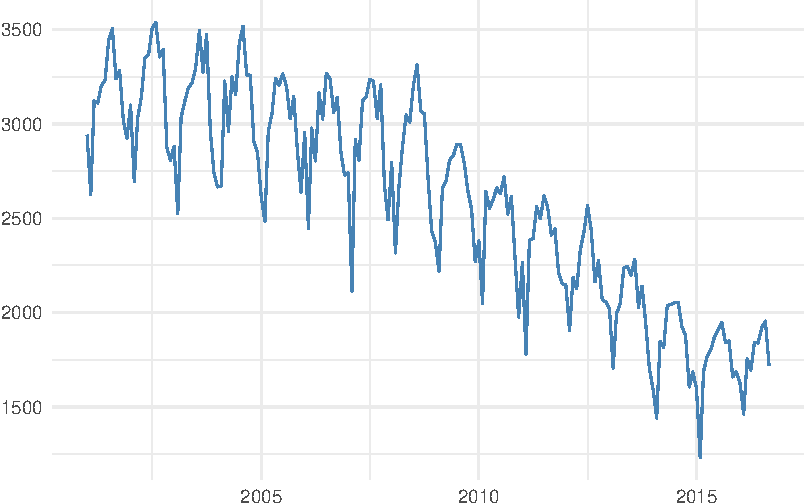
\includegraphics{Assessment_1v10_files/figure-latex/fig-1.pdf}
\caption{Crimes evolution}
\end{figure}

In Figure 2, we do the same analysis by type of crime to analyze if all
of them have followed a similar pattern. Except the deceptive practice,
which keeps in similar values as in 2001, the rest of type of crimes
have been falling to a greater or lesser extent.

\begin{figure}[H]

{\centering 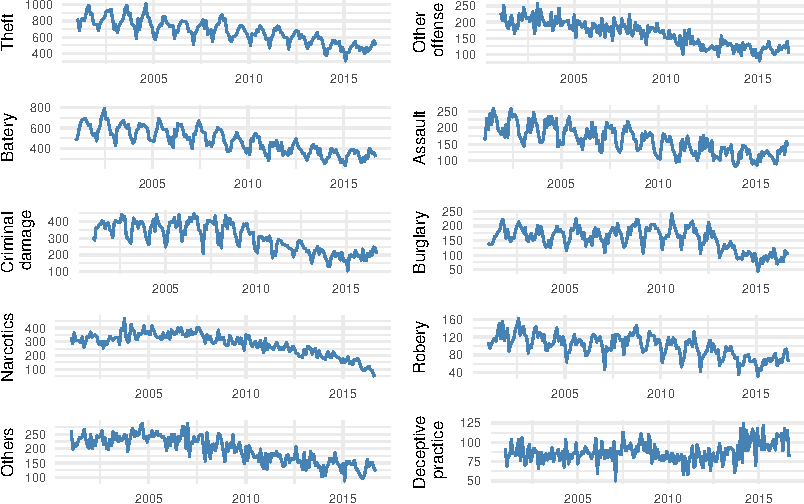
\includegraphics{Assessment_1v10_files/figure-latex/fig2-1} 

}

\caption{Evolution per type of crime}\label{fig:fig2}
\end{figure}

\subsubsection{What time of day do most types of crime
occur?}\label{what-time-of-day-do-most-types-of-crime-occur}

The peak hour of crimes morning, other crimes peak during the and the
final group of crimes peak at night.

\begin{figure}[H]

{\centering 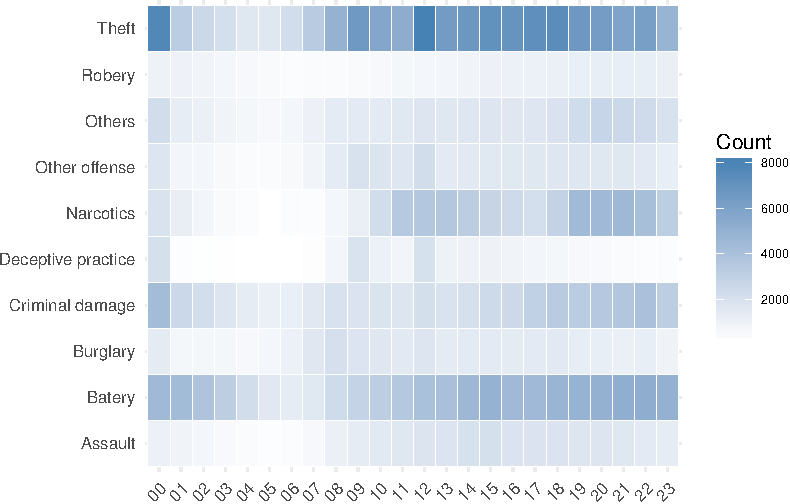
\includegraphics{Assessment_1v10_files/figure-latex/fig9-1} 

}

\caption{Type of crime vs hour}\label{fig:fig9}
\end{figure}

\subsubsection{In which locations are specific types of crime more
likely to
happen?}\label{in-which-locations-are-specific-types-of-crime-more-likely-to-happen}

In figure 4, we can see that some locations are more likely per type of
crime. For theft for instance it is better this or that.

\begin{figure}[H]

{\centering 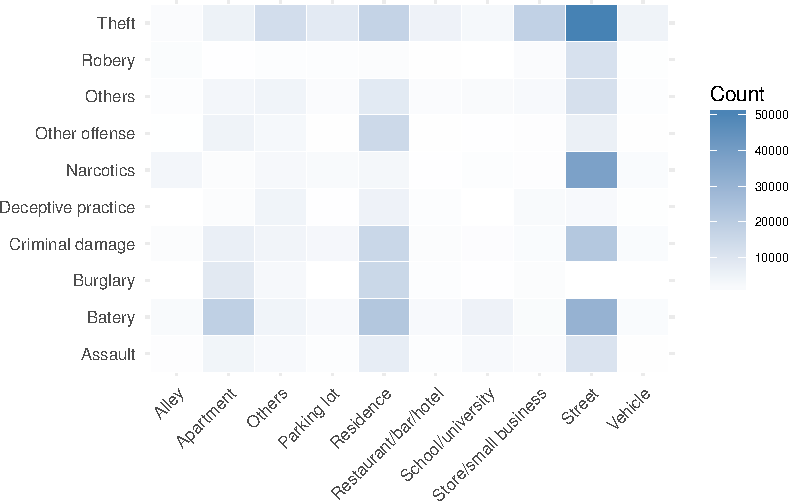
\includegraphics{Assessment_1v10_files/figure-latex/fig11-1} 

}

\caption{Type of crime vs location}\label{fig:fig11}
\end{figure}

\subsubsection{Which districts of the city are potentially more
dangerous per type of
crime?}\label{which-districts-of-the-city-are-potentially-more-dangerous-per-type-of-crime}

Finally, Figure 5 shows the districts which are more potentially
dangerous per tyep of crime. District 11 for instance seems clearly
problematic for Narcotics.

\begin{figure}[H]

{\centering 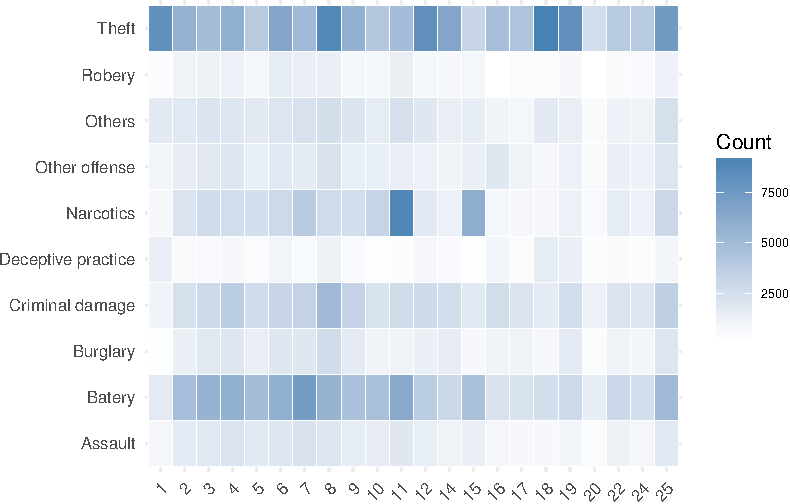
\includegraphics{Assessment_1v10_files/figure-latex/fig10-1} 

}

\caption{Type of crime vs district}\label{fig:fig10}
\end{figure}

\section{Conclusions}\label{conclusions}


\end{document}
